%%%%%%%%%%%%%%%%%%%%%%%%%%%%%%%%%%%%%%%%%
% Beamer Presentation
% LaTeX Template
% Version 1.0 (10/11/12)
%
% This template has been downloaded from:
% http://www.LaTeXTemplates.com
%
% License:
% CC BY-NC-SA 3.0 (http://creativecommons.org/licenses/by-nc-sa/3.0/)
%
%%%%%%%%%%%%%%%%%%%%%%%%%%%%%%%%%%%%%%%%%

%----------------------------------------------------------------------------------------
%	PACKAGES AND THEMES
%----------------------------------------------------------------------------------------

\documentclass{beamer}

\mode<presentation> {

% The Beamer class comes with a number of default slide themes
% which change the colors and layouts of slides. Below this is a list
% of all the themes, uncomment each in turn to see what they look like.

%\usetheme{default}
%\usetheme{AnnArbor}
%\usetheme{Antibes}
%\usetheme{Bergen}
%\usetheme{Berkeley}
%\usetheme{Berlin}
%\usetheme{Boadilla}
%\usetheme{CambridgeUS}
%\usetheme{Copenhagen}
%\usetheme{Darmstadt}
%\usetheme{Dresden}
%\usetheme{Frankfurt}
%\usetheme{Goettingen}
%\usetheme{Hannover}
%\usetheme{Ilmenau}
%\usetheme{JuanLesPins}
%\usetheme{Luebeck}
\usetheme{Madrid}
%\usetheme{Malmoe}
%\usetheme{Marburg}
%\usetheme{Montpellier}
%\usetheme{PaloAlto}
%\usetheme{Pittsburgh}
%\usetheme{Rochester}
%\usetheme{Singapore}
%\usetheme{Szeged}
%\usetheme{Warsaw}

% As well as themes, the Beamer class has a number of color themes
% for any slide theme. Uncomment each of these in turn to see how it
% changes the colors of your current slide theme.

%\usecolortheme{albatross}
%\usecolortheme{beaver}
%\usecolortheme{beetle}
%\usecolortheme{crane}
%\usecolortheme{dolphin}
%\usecolortheme{dove}
%\usecolortheme{fly}
%\usecolortheme{lily}
%\usecolortheme{orchid}
%\usecolortheme{rose}
%\usecolortheme{seagull}
%\usecolortheme{seahorse}
%\usecolortheme{whale}
%\usecolortheme{wolverine}

%\setbeamertemplate{footline} % To remove the footer line in all slides uncomment this line
%\setbeamertemplate{footline}[page number] % To replace the footer line in all slides with a simple slide count uncomment this line

%\setbeamertemplate{navigation symbols}{} % To remove the navigation symbols from the bottom of all slides uncomment this line
}

\usepackage{graphicx} % Allows including images
\usepackage{booktabs} % Allows the use of \toprule, \midrule and \bottomrule in tables

%----------------------------------------------------------------------------------------
%	TITLE PAGE
%----------------------------------------------------------------------------------------

\title[HULA]{\textit{Paper Presentation on}\\ \textit{``HULA: Scalable Load Balancing using Programmable Data-Planes"}} % The short title appears at the bottom of every slide, the full title is only on the title page

\author{Naga Ganesh Kurapati} % Your name
\institute[UMass Lowell] % Your institution as it will appear on the bottom of every slide, may be shorthand to save space
{
EECE.7290 Selected Topics on Software Defined Networking \\
\medskip
University of Massachusetts Lowell \\ % Your institution for the title page
\medskip
\text{Instructor: Prof.Yan Luo} % Your email address
}
\date{\today} % Date, can be changed to a custom date

\begin{document}

\begin{frame}
\titlepage % Print the title page as the first slide
\end{frame}

\begin{frame}
\frametitle{Overview} % Table of contents slide, comment this block out to remove it
\tableofcontents % Throughout your presentation, if you choose to use \section{} and \subsection{} commands, these will automatically be printed on this slide as an overview of your presentation
\end{frame}

%----------------------------------------------------------------------------------------
%	PRESENTATION SLIDES
%----------------------------------------------------------------------------------------

%------------------------------------------------
\section{Background} % Sections can be created in order to organize your presentation into discrete blocks, all sections and subsections are automatically printed in the table of contents as an overview of the talk
%------------------------------------------------

\subsection{Traditionally, How routing is done?} % A subsection can be created just before a set of slides with a common theme to further break down your presentation into chunks

\begin{frame}
\frametitle{Traditionally, How routing is done?}
\begin{columns}[T] % contents are top vertically aligned
	\begin{column}[T]{7.5cm} 
		\begin{itemize}
			\item Distributed protocols like OSPF, RIP etc. are used to discover routes
			\item They run periodically to gather the information about link states and then processed to decide the route
			\item When one of link fails, this protocols can update the information with in seconds. And new route is calculated.
			\item Over the few decades it is widely accepted by different vendors
			\item Network operators have no access to modify the behavior to do things like traffic engineering
		\end{itemize}
	\end{column}
	\begin{column}[T]{5cm} 
		\begin{figure}
			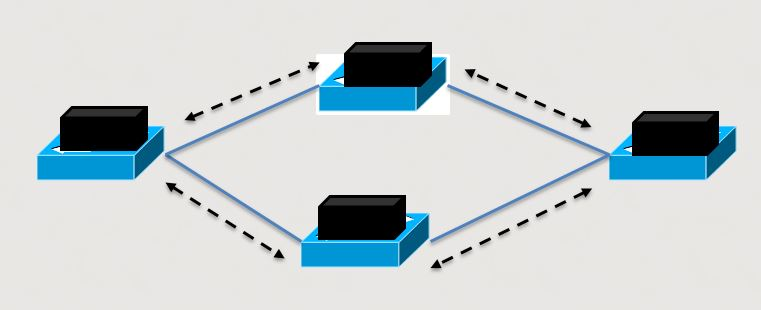
\includegraphics[scale=0.25]{1}
			\caption{Traditional Network}
		\end{figure}
	\end{column}
\end{columns}
\medskip
\textcolor{red}{RELIABLE, MOSTLY ADOPTED. BUT NOT FLEXIBLE.}
\end{frame}

%------------------------------------------------
\subsection{Software-Defined Networking, What it is promising?}

\begin{frame}
	\frametitle{Software-Defined Networking, What it is promising?}
	\begin{columns}[T] % contents are top vertically aligned
		\begin{column}[T]{7.5cm} 
			Decoupled Data plane and control plane.
			\begin{enumerate}
				\item Centralized view of the network
				\item Simpler data plane(header matching). Functionality of the switch is abstracted
				\item Unified control interface like OpenFlow
			\end{enumerate}
		\end{column}
		\begin{column}[T]{5cm} 
			\begin{figure}
				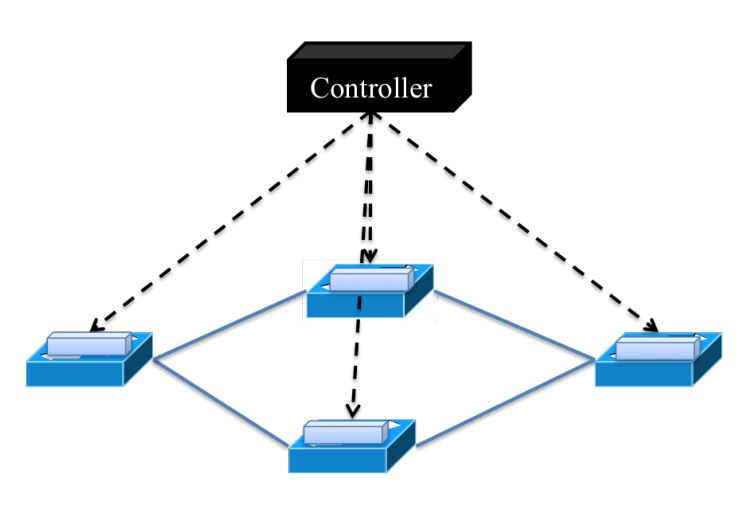
\includegraphics[scale=0.25]{2}
				\caption{Software-Defined Networking}
			\end{figure}
		\end{column}
	\end{columns}
	\medskip
	\textcolor{red}{RELIABLE, FLEXIBLE AND EFFICIENT!!! HOW?}
\end{frame}

%------------------------------------------------
\subsection{Understanding the parameters}

\begin{frame}
	\frametitle{Understanding the parameters}
		\begin{enumerate}
			\item Efficiency: Multiple paths for connecting network end points(Useful for diverting traffic). Avoid congestion when operating at high utilization.Efficient use of Underlying network bandwidth.\textcolor{red}{Better Load Balancing}
			\item Flexibility: Flexible enough to accommodate different control plane rules. \textcolor{red}{Sometimes larger set of rules and also lookup should be fast enough}
			\item Reliability: What if single central controller fails?  \textcolor{red}{Fault Tolerance}
		\end{enumerate}
\end{frame}

%------------------------------------------------
\subsection{Challenges faced by SDN}

\begin{frame}
	\frametitle{Challenges faced by SDN}
	\begin{figure}
		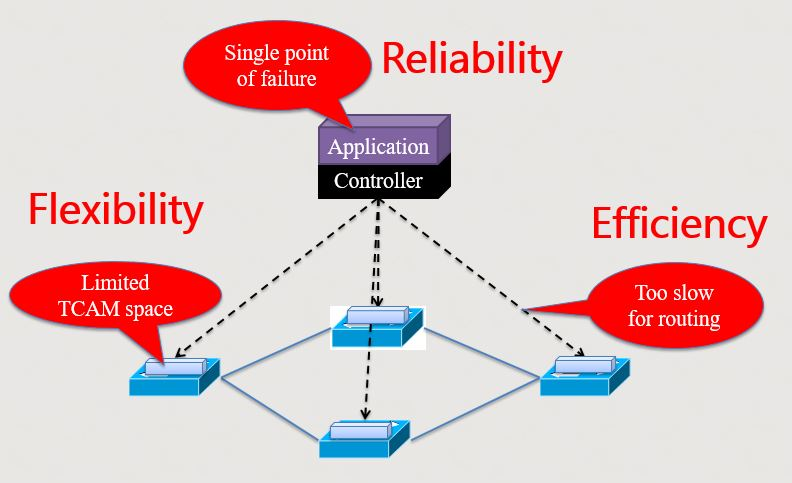
\includegraphics[width=0.8\linewidth]{3}
	\end{figure}
\end{frame}

%------------------------------------------------
\section{Efficiency - Better Load Balancing}
\subsection{Equal-cost multi-path routing (ECMP)}
\begin{frame}
	\frametitle{Efficiency - Better Load Balancing}
	\begin{columns}[T] % contents are top vertically aligned
		\begin{column}[T]{7cm} 
			\begin{block}{Traditionally, Equal-cost multi-path routing (ECMP)}
			-- Data centers networks uses multi-rooted topologies like Leaf-Spine, Fat-Tree etc. to provide large bisection bandwidth \\
			-- Spreads traffic by randomly assigning each flow to one of several paths
			\end{block}
		\end{column}
		\begin{column}[T]{5cm} 
			\begin{figure}
				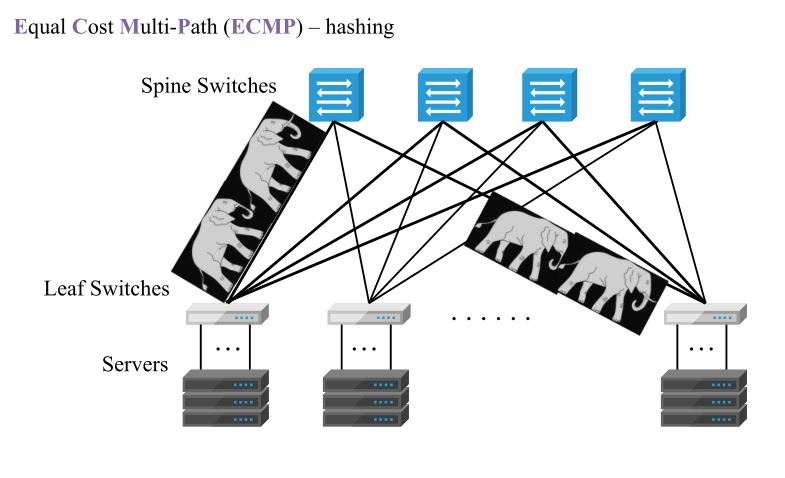
\includegraphics[scale=0.25]{4}
				\caption{ECMP}
			\end{figure}
		\end{column}
	\end{columns}
	\medskip
	\begin{itemize}
	\item\textcolor{red}{Degraded performance when two long-running flows are assigned to same path} \\
	\item\textcolor{red}{Not reactive to Link failures.Network is underutilized.Congested in asymmetric topologies}
\end{itemize}
\end{frame}

%------------------------------------------------
\subsection{SDN, Central controller to decide traffic flow}
\begin{frame}
	\frametitle{Efficiency - Better Load Balancing}
	\begin{columns}[T] % contents are top vertically aligned
		\begin{column}[T]{7cm} 
			\begin{block}{SDN, Central controller to decide traffic flow}
				--  Contoller has global visibility of congestion. Run traffic enginnering algorithms and push the commands to switches to manage traffic\\
				--  Hedera , SWAN(Microsoft) ,
				and B4(Google)
			\end{block}
		\end{column}
		\begin{column}[T]{5cm} 
			\begin{figure}
				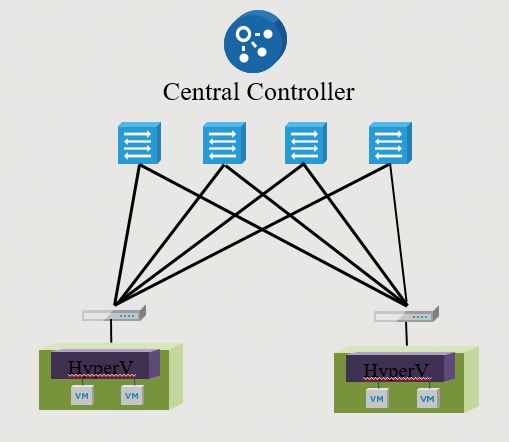
\includegraphics[scale=0.35]{5}
			\end{figure}
		\end{column}
	\end{columns}
	\medskip
	\begin{itemize}
		\item\textcolor{red}{Control plane timescales are too slow to implement load balancing to efficiently use the available network capacity} \\
		\item\textcolor{red}{Takes minutes to react for changing network conditions. Slow down the volatile traffic}
	\end{itemize}
\end{frame}

%------------------------------------------------
\subsection{CONGA: Congestion-Aware Load Balancing (Cisco)}
\begin{frame}
	\frametitle{Efficiency - Better Load Balancing}
	\begin{columns}[T] % contents are top vertically aligned
		\begin{column}[T]{7cm} 
			\begin{block}{CONGA: Congestion-Aware Load Balancing (Cisco)}
				--  Data-plane load-balancing technique  \\
				--  Load balancing decisions every few microseconds \\
				--  \textcolor{red}{Determine the entire path. Maintains forwarding state for a large number of tunnels}
			\end{block}
		\end{column}
		\begin{column}[T]{5cm} 
			\begin{figure}
				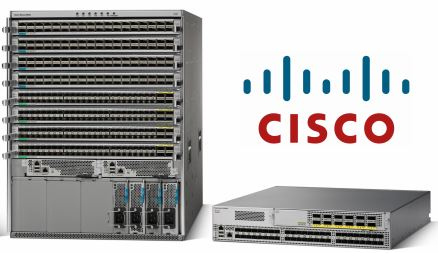
\includegraphics[scale=0.35]{6}
				\caption{CONGA}
			\end{figure}
		\end{column}
	\end{columns}
	\medskip
	\begin{itemize}
		\item\textcolor{red}{Costly, use custom silicon chip.CONGA algorithm cannot be modified, once fabricated} \\
		\item\textcolor{red}{ Maintains congestion state for every path at the leaf switches. Limited to topologies with a small number of paths like two-tier Leaf-Spine}
	\end{itemize}
\end{frame}

%------------------------------------------------
\subsection{Introduction to HULA }
\begin{frame}
	\frametitle{Efficiency -  Introduction to HULA}
	HULA - Hop-by-hop Utilization-aware Load balancing Architecture \\
	\begin{enumerate}
		\item\textcolor{red}{Topology oblivious and Scalable:} More Scalable than CONGA. Only picks next hop of globally best path to a destination.
		\item\textcolor{red}{Programmable data planes using P4:} HULA algorithm can modified and inspected as for the needs of network operator.
		\item\textcolor{red}{Congestion-aware switches:} Sends special probes periodically to gather link state information. Accumulate a table to determine next best hop towards any destination. Similar to distance vector protocol.
		\item\textcolor{red}{Fine-grained load balancing:} Break down long-running flows into \textit{flow-lets} to choose different paths to control congestion
	\end{enumerate}
\end{frame}

%------------------------------------------------
\subsection{Design Challenges for HULA}
\begin{frame}
	\frametitle{Efficiency - HULA Design Challenges}
	\begin{enumerate}
		\item\textcolor{red}{Large path utilization matrix:} Load balancing at Top of Rack switches (ToRs). Fat-Tree topology with radix
		k, then it needs to track ${k^2}$ paths for each destination ToR. For m leafs then ${m*k^2}$\\
		\textcolor{red}{More memory.Expensive!!}
		\begin{figure}
			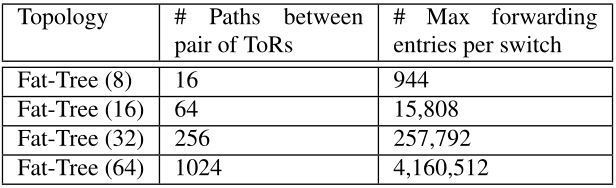
\includegraphics[width=0.6\linewidth]{7}
		\end{figure}
		\item\textcolor{red}{Large forwarding state:} Addition to above matrix, need to store large forwarding tables in each switch to support a leaf-to-leaf tunnel for each path that it needs to route packets over.
	%	\item\textcolor{red}{Discovering uncongested paths:} Sends special probes periodically to gather link state information. Accumulate a table to determine next best hop towards any destination. Similar to distance vector protocol.
	%	\item\textcolor{red}{Programmability:} Break down long-running flows into \textit{flow-lets} to choose different paths to control congestion
	\end{enumerate}
\end{frame}

%------------------------------------------------

\begin{frame}
	\frametitle{Efficiency - HULA Design Challenges}
	\begin{enumerate}
		\setcounter{enumi}{2}
			\item\textcolor{red}{Discovering uncongested paths:} At high network utilization, more number of paths exits. It takes time to discover an uncongested path
			\item\textcolor{red}{Programmability:} Tedious process for significant design and verification data-planeload-balancing schemes on hardware of switch. For modification, operator has to wait for the next product cycle.\\
			\textcolor{red}{Solution for programmability:P4}
	\end{enumerate}
\end{frame}

%------------------------------------------------

\subsection{HULAOverview: Scalable, Proactive, Adaptive, and Programmable}
\begin{frame}
	\frametitle{Efficiency - HULAOverview: Scalable, Proactive, Adaptive, and Programmable}
	\begin{enumerate}
		\item\textcolor{red}{Maintaining compact path utilization:}  Instead of maintaining path utilization for all paths to a destination ToR, a HULA switch only maintains a table that maps the destination ToR to the best next hop as measured by path utilization. Effectively removing the pressure of path explosion on switch memory.
		\item\textcolor{red}{Scalable and adaptive routing:}  HULA’s best hop table eliminates the need for separate source routing in order to exploit multiple network paths.Each switch independently chooses the best next hop to the destination
		\item\textcolor{red}{Automatic discovery of failures:} If a switch does not receive a probe from a neighboring switch for more than a certain threshold of time
	\end{enumerate}
\end{frame}

%------------------------------------------------

\begin{frame}
	\frametitle{Efficiency - HULAOverview: Scalable, Proactive, Adaptive, and Programmable}
	\begin{enumerate}
		\setcounter{enumi}{3}
		\item\textcolor{red}{Proactive path discovery:}  In HULA, probes are sent separately from data packets instead of piggybacking on them.  This way, switches can instantaneously pick an uncongested path on the arrival of a new flowlet without having to first explore congested paths
		\item\textcolor{red}{Programmability:}Processing a packet in a HULA switch involves switch state updates at line rate in the packet processing pipeline. In particular, processing a probe involves updating the best hop table and replicating the probe to neighboring switches. Processing a data packet involves reading the best hop table and updating a flowlet table if necessary.
		\item\textcolor{red}{Topology and transport oblivious:} HULA is not designed for a specific topology.
	\end{enumerate}
\end{frame}

%------------------------------------------------

\subsection{HULA Design: Probes and Flowlets}
\begin{frame}
	\frametitle{Efficiency - HULA Design: Probes and Flowlets}
	\begin{enumerate}
	\item\textcolor{red}{Origin and Replication of HULA Probes}\\
	\end{enumerate}
	-- Every ToR sends HULA probes on all the uplinks that connect it to the data-center network\\
	-- Once the probes reach A1, it will forward the probe to all the other downstream ToRs (T2) and all the upstream spines (S1, S2).\\
	-- However, when the switch A4 receives a probe from S3, it replicates it to all its downstream ToRs but not to other upstream spines S4\\
	-- This makes sure that all paths in the network are covered by the probes\\
	-- Once a probe reaches another ToR, it ends its journey\\
	\begin{figure}
		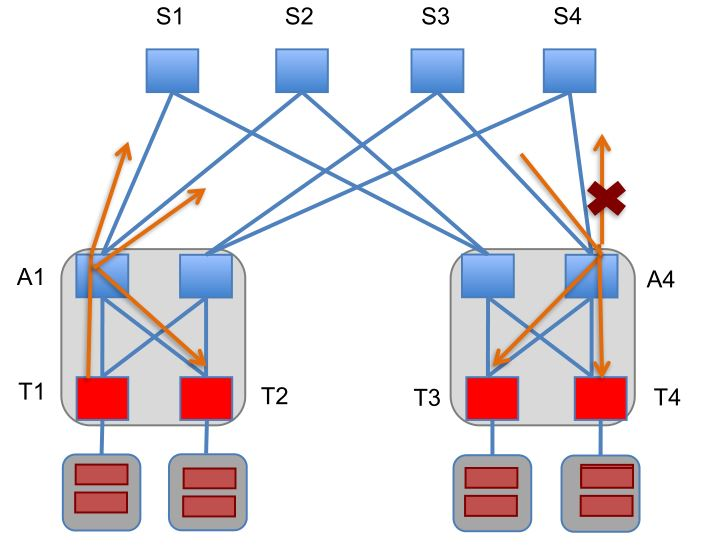
\includegraphics[width=0.36\linewidth]{8}
	\end{figure}
\end{frame}

%------------------------------------------------

\begin{frame}
	\frametitle{Efficiency - HULA Design: Probes and Flowlets}
	\begin{enumerate}
		\setcounter{enumi}{1}
		\item\textcolor{red}{Processing Probes to Update Best Path}\\
	\end{enumerate}
		\begin{figure}
			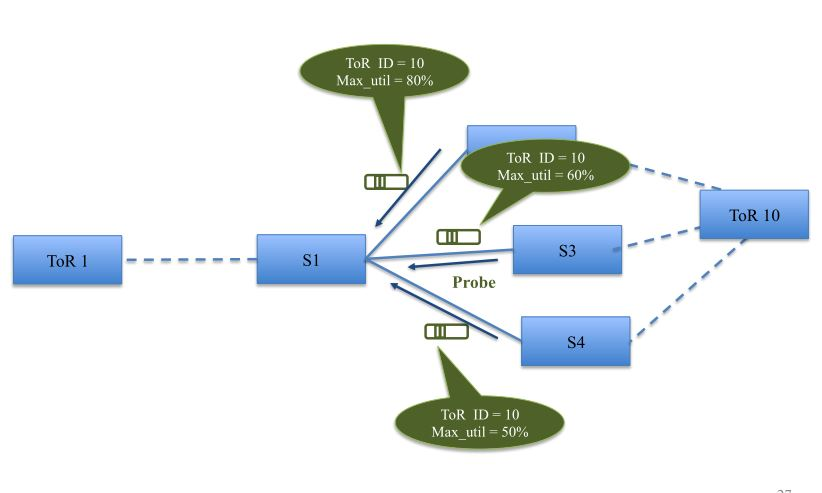
\includegraphics[width=1\linewidth]{9}
		\end{figure}
\end{frame}

%------------------------------------------------
\begin{frame}
	\frametitle{Efficiency - HULA Design: Probes and Flowlets}
	\begin{enumerate}
		\setcounter{enumi}{1}
		\item\textcolor{red}{Processing Probes to Update Best Path}\\
	\end{enumerate}
	\begin{figure}
		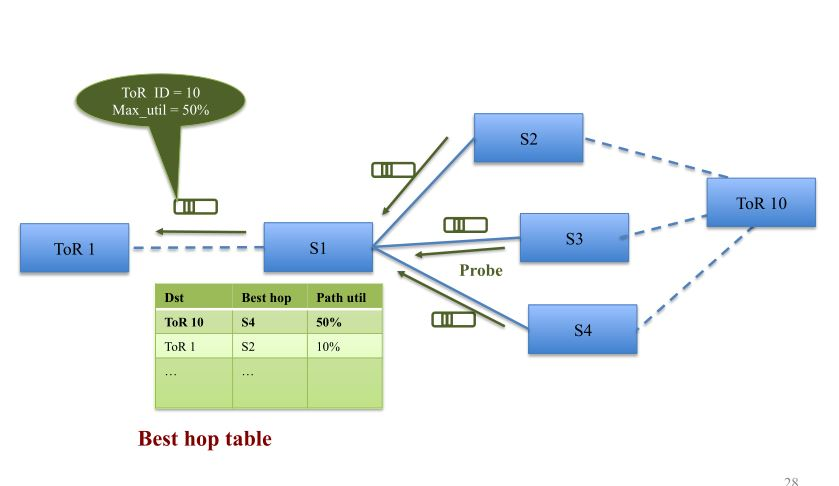
\includegraphics[width=1\linewidth]{10}
	\end{figure}
\end{frame}

%------------------------------------------------
\begin{frame}
	\frametitle{Efficiency - HULA Design: Probes and Flowlets}
	\begin{enumerate}
		\setcounter{enumi}{1}
		\item\textcolor{red}{Processing Probes to Update Best Path}\\
	\end{enumerate}
	\begin{figure}
		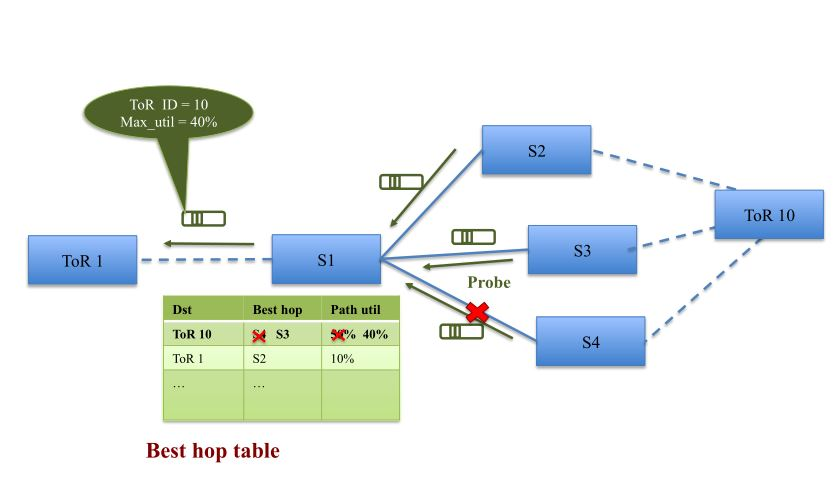
\includegraphics[width=1\linewidth]{11}
	\end{figure}
\end{frame}

%------------------------------------------------
\begin{frame}
	\frametitle{Efficiency - HULA Design: Probes and Flowlets}
	\begin{enumerate}
		\setcounter{enumi}{1}
		\item\textcolor{red}{Processing Probes to Update Best Path}\\
	\end{enumerate}
	\begin{figure}
		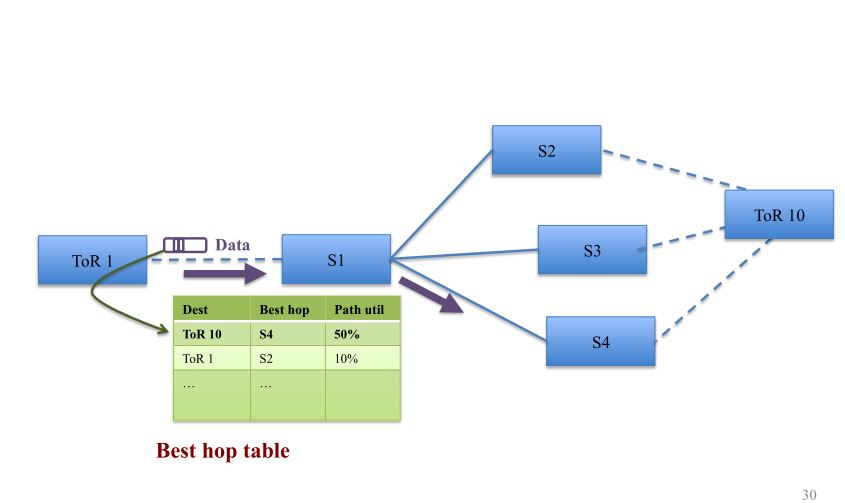
\includegraphics[width=1\linewidth]{12}
	\end{figure}
\end{frame}

%------------------------------------------------
\begin{frame}
	\frametitle{Efficiency - HULA Design: Probes and Flowlets}
	\begin{enumerate}
		\setcounter{enumi}{1}
		\item\textcolor{red}{Processing Probes to Update Best Path}\\
	\end{enumerate}
	\begin{figure}
		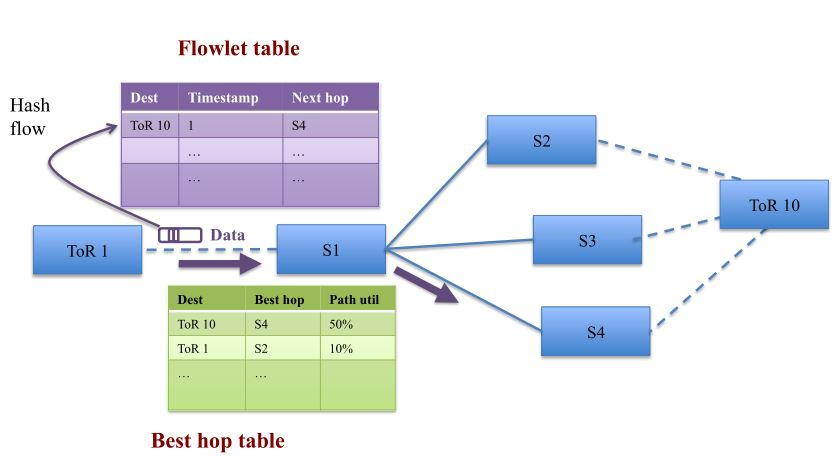
\includegraphics[width=1\linewidth]{13}
	\end{figure}
\end{frame}

%------------------------------------------------
\begin{frame}
	\frametitle{Efficiency - HULA Design: Probes and Flowlets}
	\begin{enumerate}
		\setcounter{enumi}{1}
		\item\textcolor{red}{Processing Probes to Update Best Path}\\
	\end{enumerate}
	\begin{itemize}
		\item Utilization Estimator. U = ${ D + U \times (1 - \frac{\Delta t}{\tau})}$ \\
		U is the link utilization estimator \\
		D is the size of the outgoing packet that triggered the update for the estimator\\
		${\Delta t}$ is the amount of time passed since the last update to the estimator\\
		${\tau}$is a time constant
	\end{itemize}
\end{frame}

%------------------------------------------------

\begin{frame}
	\frametitle{Efficiency - HULA Design: Probes and Flowlets}
	\begin{enumerate}
		\setcounter{enumi}{2}
		\item\textcolor{red}{Flowlet Forwarding on Best Paths}\\
	\end{enumerate}
	\begin{itemize}
		\item HULA load balances at the granularity of flowlets in order to avoid packet reordering in TCP
		\item  A flowlet is detected by a switch whenever the inter-packet gap (time interval between the arrival of two consecutive packets) in a flow is greater than a flowlet threshold Tf
		\item  Use flow table to keep track of all flowlets. 
	\end{itemize}
\end{frame}

%------------------------------------------------

\begin{frame}
	\frametitle{Efficiency - HULA Design: Probes and Flowlets}
	\begin{enumerate}
		\setcounter{enumi}{3}
		\item\textcolor{red}{Data-Plane Adaptation to Failures}\\
	\end{enumerate}
	\begin{itemize}
		\item HULA also learns about link failures from the absence of probes
		\item The data plane implements an aging mechanism for the entries in best Hop table.
		\item  HULA tracks the last time bestHop was updated using an updateTime table. If a bestHop entry for a destination ToR is not refreshed within the last Tfail (a threshold for detecting failures), then any other probe that carries information about this ToR (from a different hop) will simply replace the bestHop and pathUtil entries for the ToR 
		\item  HULA does not need to rely on the control plane to detect and adapt to failures. And it is faster
	\end{itemize}
\end{frame}

%------------------------------------------------

\begin{frame}
	\frametitle{Efficiency - HULA Design: Probes and Flowlets}
	\begin{enumerate}
		\setcounter{enumi}{4}
		\item\textcolor{red}{Probe Overhead and Optimization}\\
	\end{enumerate}
	\begin{itemize}
		\item \textcolor{red}{Setting probe frequency:}The network switches only use the congestion information to make load balancing decisions when a new flowlet arrives at the switch(CONGA).
		\item \textcolor{red}{Optimization for probe replication:}HULA maintains a lastSent table indexed by ToR IDs to avoid probe redundancy.Only one probe is sent by A to B within a time window of Tp  
		\item \textcolor{red}{Overhead:} probe overhead on any given network link = ${\frac{probeSize\times numToRs\times100}{probeFreq\times linkBandwidth}}$\\
		probeSize is 64 bytes, numTors is the total number of leaf ToRs supported in the network and probeFreq is the HULA probe frequency.\\
		Therefore, in a network with 40G links supporting a total of 1000 ToRs, with probe frequency of 1ms, the overhead comes to be 1.28\%.
	\end{itemize}
\end{frame}

%------------------------------------------------

\subsection{Programming HULA in P4}
\begin{frame}
	\frametitle{Efficiency - Programming HULA in P4}
	\begin{figure}
		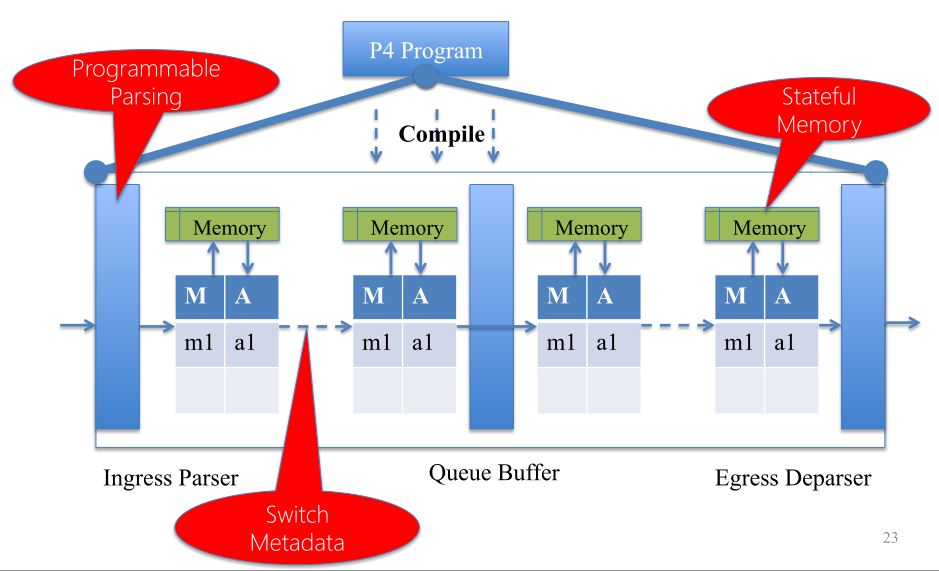
\includegraphics[width=1\linewidth]{14}
	\end{figure}
\end{frame}

%------------------------------------------------
\begin{frame}
	\frametitle{Efficiency - Programming HULA in P4}
		\begin{itemize}
			\item\textcolor{red}{HULA header format and control flow}\\
		\end{itemize}
		\begin{columns}[T] % contents are top vertically aligned
			\begin{column}[T]{6cm} 
	\begin{figure}
		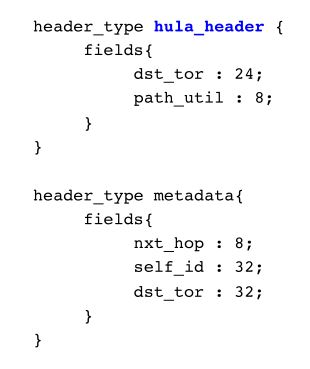
\includegraphics[width=0.7\linewidth]{15}
	\end{figure}
\end{column}
\begin{column}[T]{6.5cm} 
		\begin{figure}
			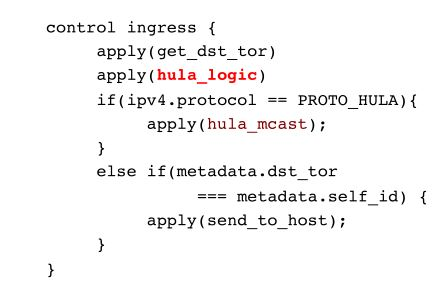
\includegraphics[width=1\linewidth]{16}
		\end{figure}
	\end{column}
\end{columns}
\end{frame}

%------------------------------------------------
\begin{frame}
	\frametitle{Efficiency - Programming HULA in P4}
	\begin{itemize}
		\item\textcolor{red}{HULA stateful packet process in P4}\\
	\end{itemize}
	
			\begin{figure}
				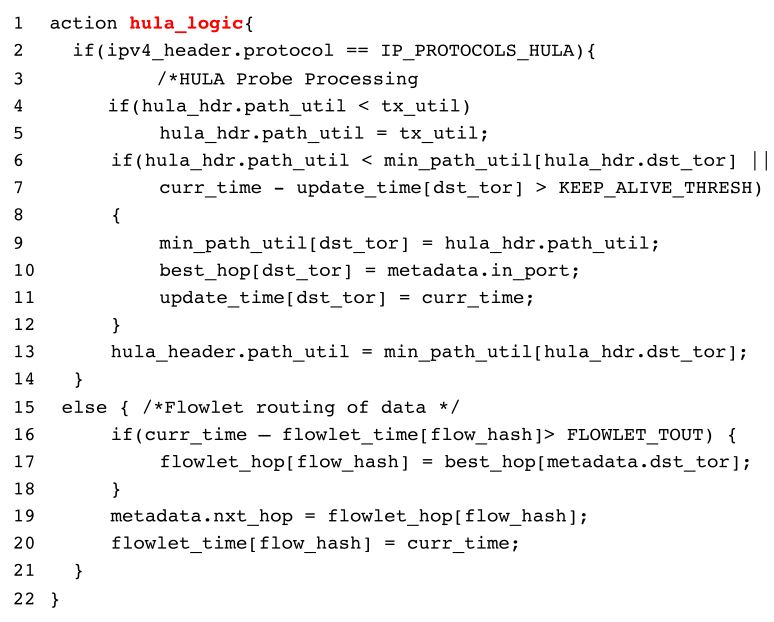
\includegraphics[width=0.75\linewidth]{17}
			\end{figure}
\end{frame}

%------------------------------------------------
 \subsection{Evaluation of HULA}
 \begin{frame}
 	\frametitle{Efficiency - Evaluation of HULA}
 	
 	\begin{figure}
 		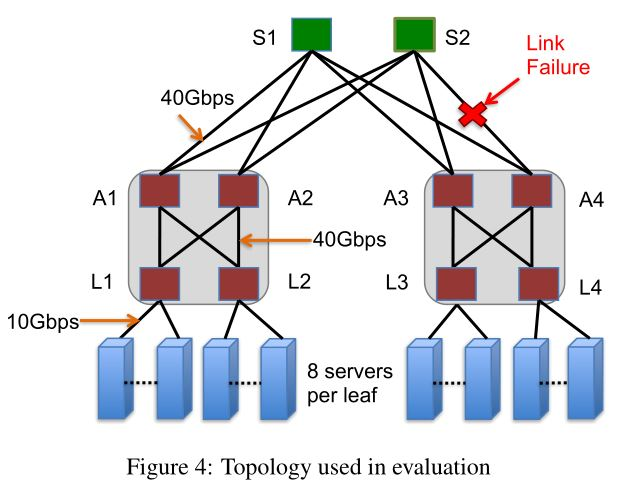
\includegraphics[width=0.8\linewidth]{18}
 	\end{figure}
 \end{frame}
 
 %------------------------------------------------
 
 \begin{frame}
 	\frametitle{Efficiency - Evaluation of HULA}
 	
 	\begin{figure}
 		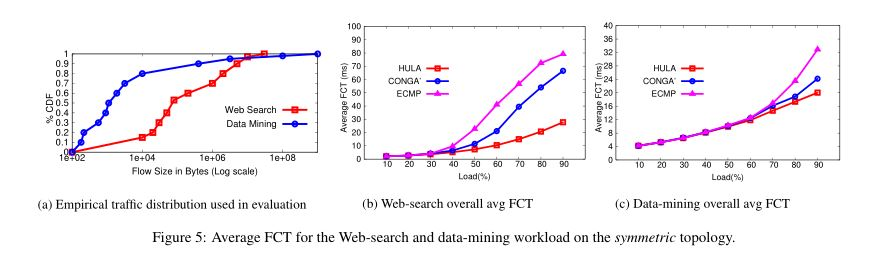
\includegraphics[width=1.05\linewidth]{19}
 	\end{figure}
 \end{frame}
 
 %------------------------------------------------
 
  \begin{frame}
  	\frametitle{Efficiency - Evaluation of HULA}
  	
  	\begin{figure}
  		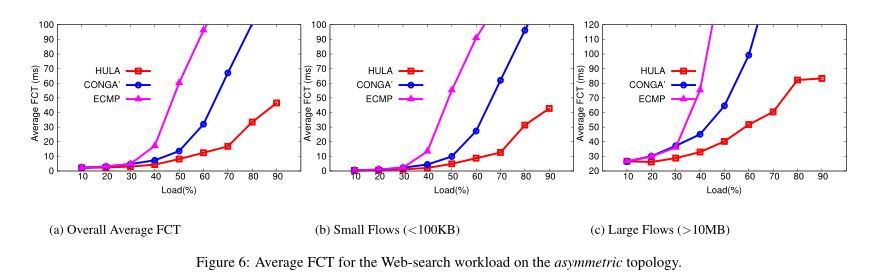
\includegraphics[width=1.05\linewidth]{20}
  	\end{figure}
  \end{frame}
  
  %------------------------------------------------
  
   \begin{frame}
   	\frametitle{Efficiency - Evaluation of HULA}
   	
   	\begin{figure}
   		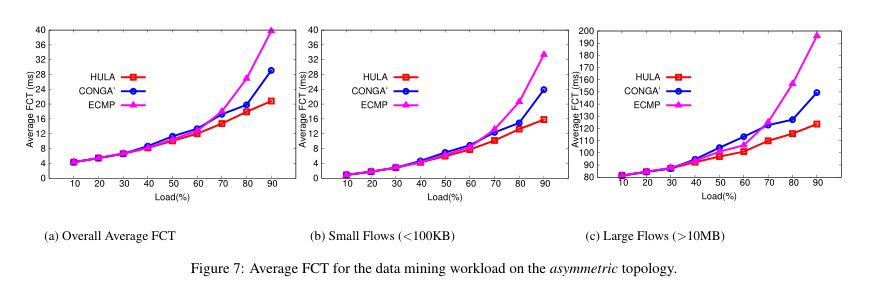
\includegraphics[width=1.05\linewidth]{21}
   	\end{figure}
   \end{frame}
   
   %------------------------------------------------
   
    \begin{frame}
    	\frametitle{Efficiency - Evaluation of HULA}
    	
    	\begin{figure}
    		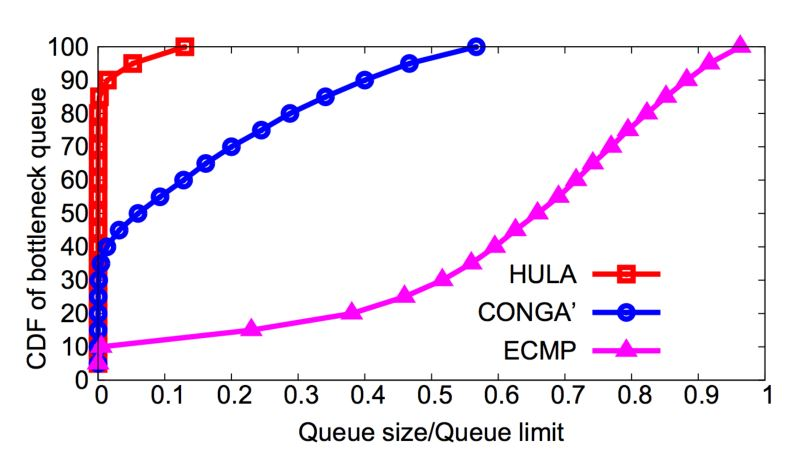
\includegraphics[width=1.05\linewidth]{22}
    	\end{figure}
    \end{frame}
    
    %------------------------------------------------
   \begin{frame}
   	\frametitle{Efficiency - Evaluation of HULA}
   	Flexibility
   	\footnotesize{
   		\begin{thebibliography}{99} % Beamer does not support BibTeX so references must be inserted manually as below
   			\bibitem[Smith, 2012]{p1} Naga Katta, Omid Alipourfard,Jennifer Rexford and David Walker 
   			\newblock CacheFlow: Dependency-Aware Rule-Caching for Software-Defined Networks
   			Proceedings of the Symposium on SDN Research,
   			\newblock \emph{Proceedings of the Symposium on SDN Research}
   		\end{thebibliography}
   	}
   	Reliability
   	\footnotesize{
   		\begin{thebibliography}{99} % Beamer does not support BibTeX so references must be inserted manually as below
   			\bibitem[Smith, 2012]{p1} Naga Katta
   			\newblock Building Efficient and Reliable Software-Defined Networks
   			\newblock \emph{ PhD. Dissertation,Princeton University}
   		\end{thebibliography}
   	}
   \end{frame}
   
   %------------------------------------------------
   
\begin{frame}
\frametitle{References}
\footnotesize{
\begin{thebibliography}{99} % Beamer does not support BibTeX so references must be inserted manually as below
\bibitem[Smith, 2012]{p1} Naga Katta, Mukesh Hira, Changhoon Kim, Anirudh Sivaraman, Jennifer Rexford, March 14-15, 2016, Santa Clara, CA, USA
\newblock HULA: Scalable Load Balancing Using
Programmable Data Planes
 Proceedings of the Symposium on SDN Research,
\newblock \emph{Proceedings of the Symposium on SDN Research}
\end{thebibliography}
\begin{thebibliography}{99} % Beamer does not support BibTeX so references must be inserted manually as below
	\bibitem[Smith, 2012]{p1} Naga Katta
	\newblock Building Efficient and Reliable Software-Defined Networks
	\newblock \emph{ PhD. Dissertation,Princeton University}
\end{thebibliography}
}
\end{frame}

%------------------------------------------------

\begin{frame}
\Huge{\centerline{Questions?}}
\end{frame}

%----------------------------------------------------------------------------------------

\end{document} 